\documentclass{article}

\usepackage{amsmath}   %% for \cfrac
\usepackage{xcolor}    %% for colored text
\usepackage{pagecolor} %% for dark background
\usepackage{graphicx}  %% for images
\usepackage{geometry}
\usepackage{hyperref}
\usepackage{wrapfig}

\geometry{
a4paper,
total={170mm,257mm},
left=20mm,
right=20mm,
top=20mm
}

\graphicspath{ {../../docs/},{../../../../docs/} }

\pagecolor{black}
\definecolor{magenta}{RGB}{255,0,255}
\definecolor{cyan}{RGB}{0,255,255}
\definecolor{white}{RGB}{255,255,255}
\definecolor{blue}{RGB}{0,0,255}
\definecolor{green}{RGB}{0,255,0}

\begin{document}

\font\titlefont=cmr12 at 30pt

\color{magenta}
\Huge{\title{\vspace{-3cm}\color{magenta}\titlefont Astrodynamics with Python}}
\color{white}
\author{Alfonso Gonzalez}
\date{}
\maketitle

\begin{center}
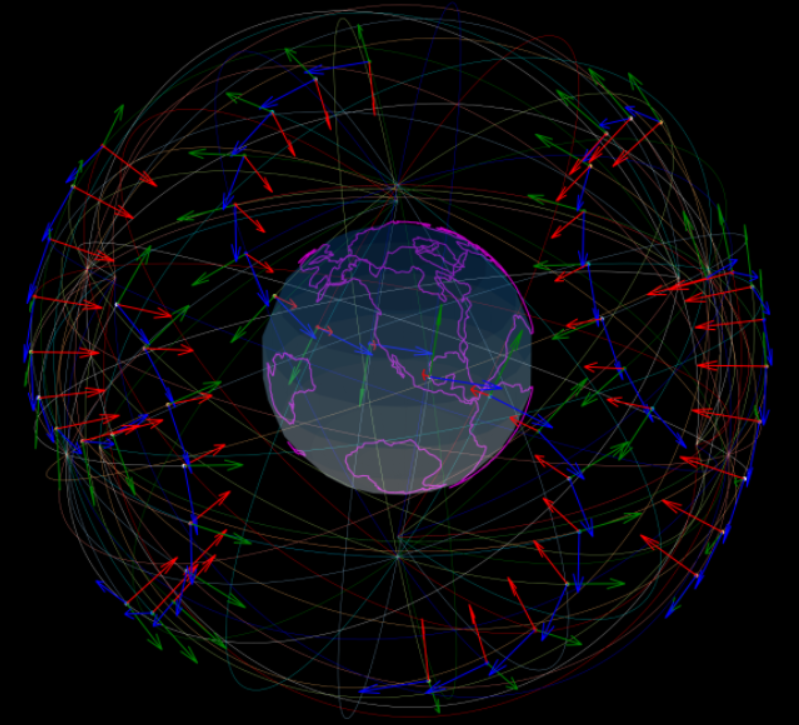
\includegraphics[width=300pt]{prof-pic-hq-centered.png}
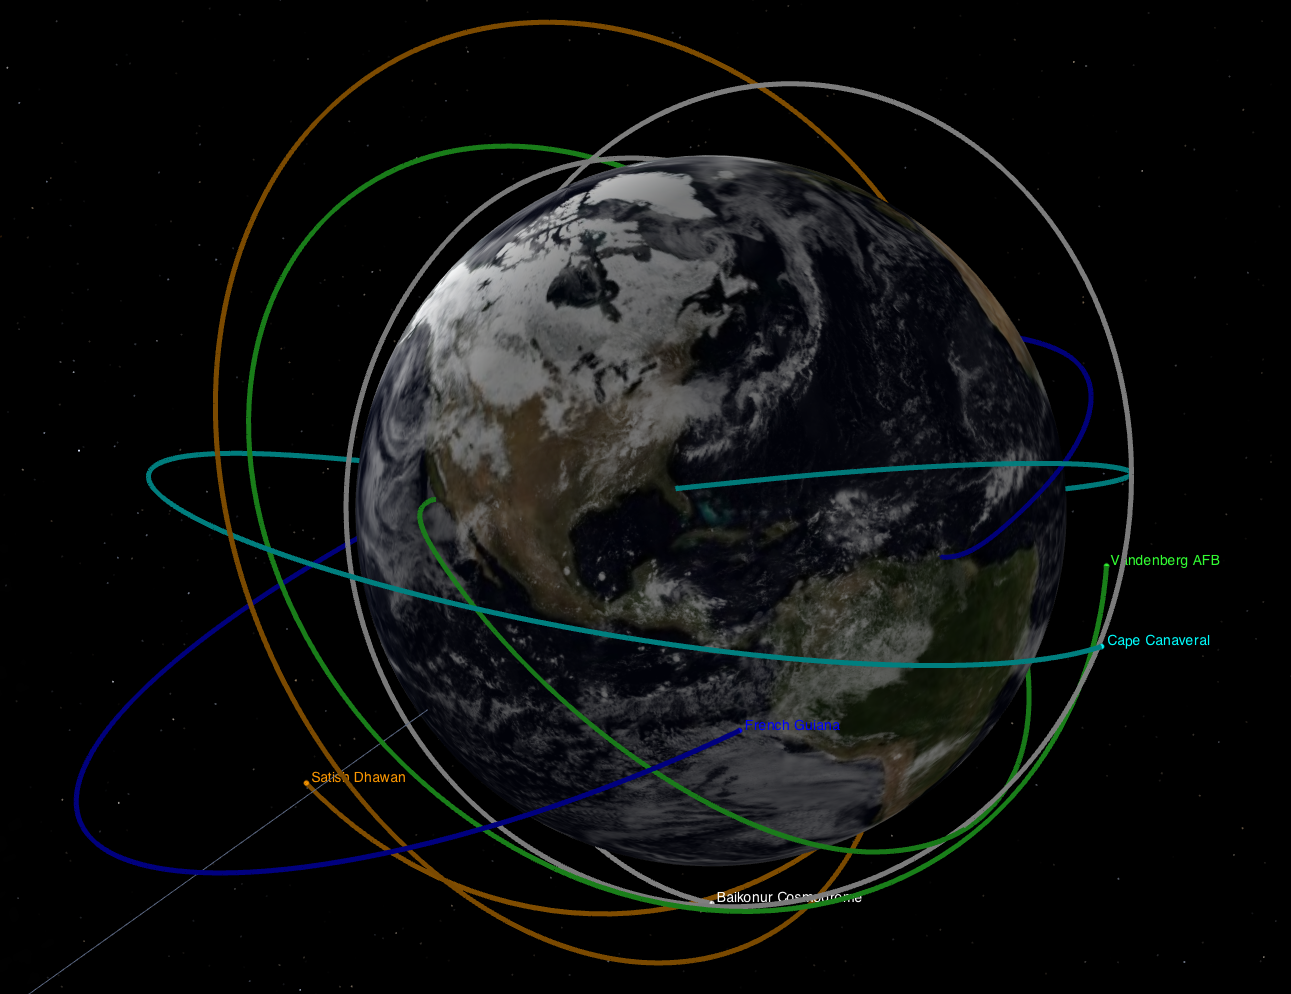
\includegraphics[width=400pt]{cosmo-3d-launches.png}
\end{center}

\newpage

\begin{center}\huge{
\color{magenta}
\hspace{-10pt}
\vfill
To: Mom (Veronica), Dad (Carl), Brother (Alberto) and all past, present, and future humans of Earth, Earth's Moon, Mars, and Beyond. Original writing began in year 2021.
\hspace{15pt}
\vfill
}
\end{center}

\newpage

\textwidth=700pt

\normalsize

\tableofcontents

\newpage

\section{Preface}

The \color{magenta}Astrodynamics with Python \color{white} book, YouTube videos, and GitHub repository are all products
of the simple belief that all information should be free to anyone with access to the internet.
They are collectively my attempt at providing useful information to the world.


Also because of that belief, if you'd like to help me by translating this project to your native language, don't hesitate
to contact me at: \color{magenta}spaceengineeringpodcast@gmail.com \color{white}


This book is unlike other books, given that (for now) it is solely electronic, is being released as its being written (chapter by chapter),
and will be a very iterative process (hence why it is being version controlled via Git). This is for multiple reasons:
\begin{itemize}
	\item Free to anyone with access to the internet
	\item Easy to publish (git push, merge to main)
	\item This is a collaboration with other engineers who contribute by translating
	\item This is a collaboration with readers (you)
	\begin{itemize}
		\item If you see a mistake or are confused by an explanation, reach out
		via email or open up Git Issue, so that when the book is updated, your
		Git Issue will be attached to the fix/improvement git commit, thus you will have
		directly contributed to this project!
		\item This applies to the book as well as the software in this repository.
	\end{itemize}
\end{itemize}

Now lets get to the technical work.

\section{Chapters and Material}
The following are general guidelines of how this book will be written:
\begin{itemize}
	\item Visuals and software will be at the center of every explanation / derivation
	\begin{itemize}
		\item In general, I don't consider myself to truly understand a problem until I can solve it on paper \textbf{AND} implement it in software.
	\end{itemize}

\end{itemize}

\noindent
The current plan is to separate the book by the following topics:
\begin{itemize}
	\item Orbital mMchanics
	\item Rocket Trajectories
	\item Numerical Methods
	\item Spacecraft Attitude Control
	\item Trajectory Optimization / Optimal Control
	\item SPICE
	\item Prerequisites
\end{itemize}
 
The book, videos, and software will all be complementing each other, and will be
continuously updated as needed / requested from the readers.

\newpage

\begin{wrapfigure}{R}{0.3\textwidth}
\centering
\includegraphics[width=0.25\textwidth]{two-body-with-coastlines.png}
\includegraphics[width=0.25\textwidth]{groundtracks.png}
\includegraphics[width=0.25\textwidth]{earth2mars.png}
\includegraphics[width=0.25\textwidth]{EVME.png}
\end{wrapfigure}

\subsection{Orbital Mechanics}
This section of the book will be organized in the same order as the
Fundamentals of Orbital Mechanics video series \color{cyan}
\href{https://www.youtube.com/playlist?list=PLOIRBaljOV8hBJS4m6brpmUrncqkyXBjB}{(link to YouTube playlist)}\color{white}

\noindent
The following are the planned topics:

\begin{itemize}
	\item The two-body problem / Newton's universal law of gravitation \color{cyan}\href{https://youtu.be/nJ_f1h49jfM}{(link)} \color{white}
	\item Ordinary differential equations (ODEs) \color{cyan}\href{https://youtu.be/8-SyHZb7w40}{(link)} \color{white}
	\item Introduction to ODE solvers (Runge-Kutta 4) \color{cyan}\href{https://youtu.be/VrH6JhIFmcA}{(link)} \color{white}
	\item Solving 2nd Order ODEs with 1st Order ODE Solvers / Propagating Orbits \color{cyan}\href{https://youtu.be/TzX6bg3Kc0E}{(link)} \color{white}
	\item Introduction to the Keplerian / Classical Orbital Elements
	\item How to Identify Keplerian Orbital Elements in 3D Orbit Plots
	\item Earth Inertial and Body Fixed Reference Frames
	\item Introduction to SPICE (Spacecraft Planet Instrument C-matrix Events)
	\item Converting between Earth Centered Inertial (EME2000) and Earth Centered Earth Fixed (IAU EARTH) Frames
	\item Groundtracks calculations
	\item How to Identify Keplerian Orbital Elements in Groundtracks Plots
	\item Two-Line Element Sets (TLEs)
	\item Hohmann Transfers
	\item Introduction to Lambert's Problem
	\item Universal Variables Lambert's Solver
	\item Interplanetary Trajectories (Synodic Periods, Earth to Mars, Earth to Jupiter, etc.)
	\item Porkchop Plots
	\item Sphere of Influence
	\item Patched Conics
	\item Gravity Assist Trajectory Design (Zero-Sphere of Influence V-Infinity Matching) \color{cyan}\href{https://youtu.be/rNpnzNKQrNg}{(link)} \color{white}
	\item Circular Restricted 3 Body Problem (CR3BP), (Lagrange Points, Invariant Manifolds, Earth-Moon Trajectories, etc.)
	\item Orbital Perturbations (J2, N-body, SRP, Higher Order Spherical Harmonics)
	\item Orbit Determination
\end{itemize}

\clearpage

\begin{wrapfigure}{R}{0.3\textwidth}
\centering
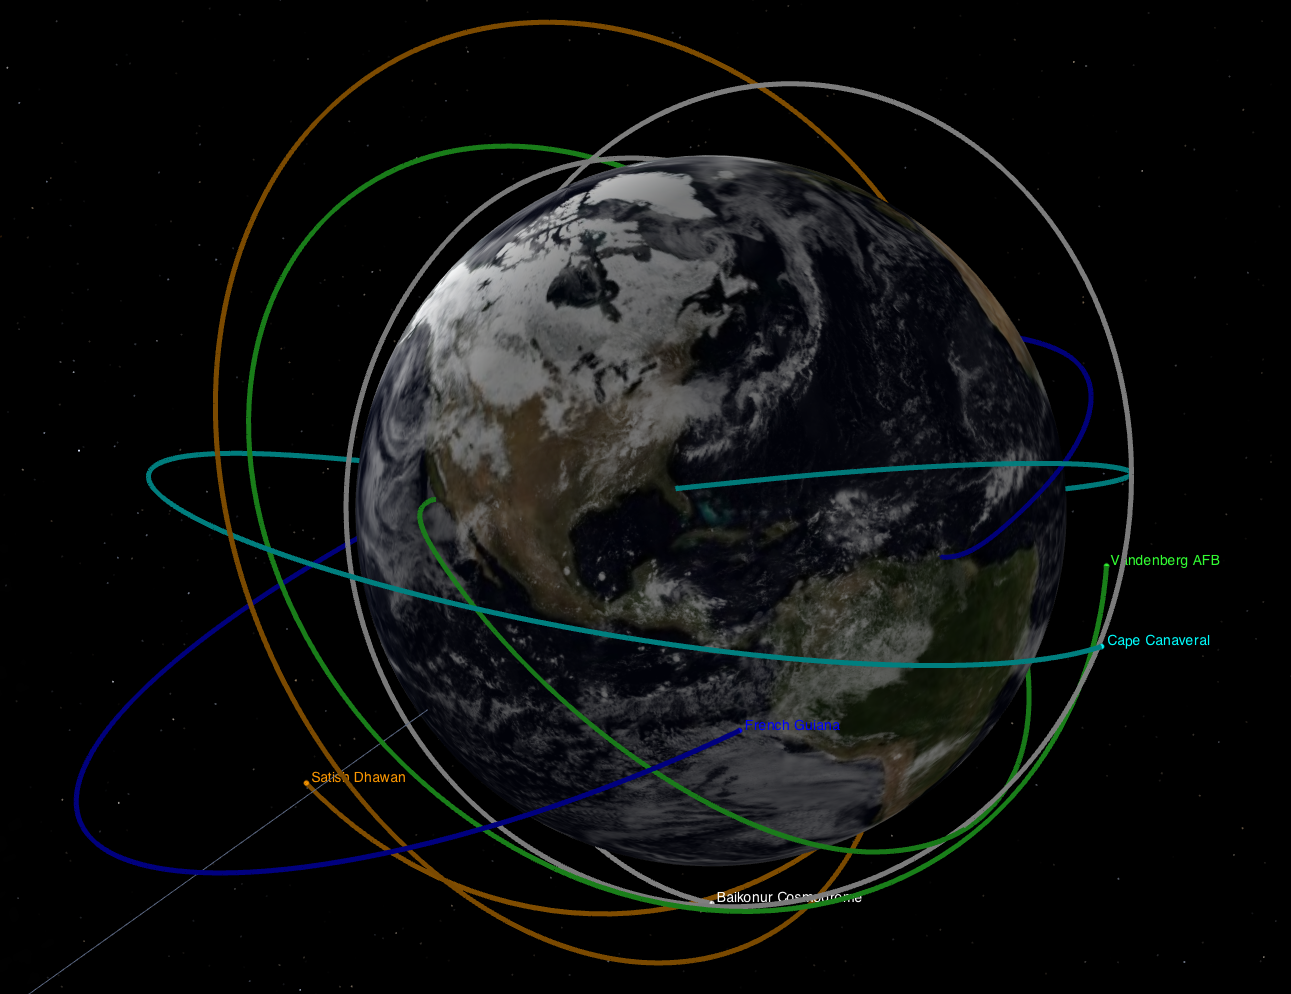
\includegraphics[width=0.25\textwidth]{cosmo-3d-launches.png}
\includegraphics[width=0.25\textwidth]{grav-turn-infos.png}
\includegraphics[width=0.25\textwidth]{max-q.png}
\includegraphics[width=0.25\textwidth]{inc-v-azimuth.png}
\includegraphics[width=0.25\textwidth]{rocket-launch-sites.png}
\end{wrapfigure}

\subsection{Rocket Trajectories}
This section of the book will be organized in the same order as the
Rocket Trajectories video series \color{cyan}
\href{https://www.youtube.com/playlist?list=PLOIRBaljOV8je0oxFAyj2o6YLXcBX1rTZ}{(link to YouTube playlist)}\color{white}

\noindent
The following are the planned topics:

\begin{itemize}
	\item Ideal Rocket Equation Derivation, Definition of Specific Impulse \color{cyan}\href{https://youtu.be/bPXjkFAnQio}{(link)} \color{white}
	\item Sounding Rocket Trajectories (1D motion) \color{cyan}\href{https://youtu.be/-4-UfoFgU0A}{(link)} \color{white}
	\item Maximum Dynamic Pressure and Aerodynamic Drag \color{cyan}\href{https://youtu.be/n74TycEj-Xc}{(link)} \color{white}
	\item Gravity Turn Rocket Trajectories (2D motion) \color{cyan}\href{https://youtu.be/n74TycEj-Xc}{(link)} \color{white}
	\item Thrust Throttling to Reduce Maximum Dynamic Pressure
	\item Introduction to Rocket Trajectories in 3D \color{cyan}\href{https://youtu.be/XZXr5BxmReQ}{(link)} \color{white}
	\item Relationship Between Launch Site Latitude, Target Orbital Inclination, and Launch Azimuth Vector
	\item Targeting Orbital Inclination from Launch Sites Around the World
	\item Calculating Inertial Velocity Vector of Rocket on Launch Pad as a Function of Latitude / Longitude Coordinates
	\item Guidance Relative to IAU EARTH (Body Fixed Frame) vs. EME2000 (Inertial Frame)
	\item Targeting Orbital Eccentricity
	\item Targeting Right Ascension (Instantaneous Launch Windows)
	\item Targeting Specific Orbits (Geostationary Transfer Orbit (GTO), ISS Rendezvous, Sun-Synchronous, etc.)
\end{itemize}

\clearpage

\subsection{Numerical Methods}
This section as of now does not directly follow any video playlists, but videos will be made as this section gets written that corresponds to the material. For now though there is still a Numerical Methods with Python \color{cyan}\href{https://www.youtube.com/playlist?list=PLOIRBaljOV8gMqhggseSHI9u2pldGZonA}{playlist}\color{white}.


\noindent
Also, there are lots of topics in this playlist that will be pre-requisities to the other sections of this book, and will be referenced from those sections.


\noindent
The following are the planned topics:

\begin{itemize}
	\item Derivative Estimations by Finite Differences
	\item Single Variable Root Solving Methods (Newton, Secant)
	\item Principal Rotation Matrices (X,Y,Z Rotations)
	\item Active vs Passive Rotation Matrices (Transposes)
	\item Axes of Rotation
	\item Euler Angles (with Matrices)
	\item Quaternions
	\item Converting Between Axes of Rotation, Rotation Matrices, and Quaternions
	\item Inertial and Non-Inertial Reference Frames
	\item Jacobian Matrix
	\item Newton Root Solver Method for Multivariable Functions (uses Jacobian)
	\item Numerically Calculate Jacobian Matrix
	\item Partial Derivatives for Multivariable Functions
	\item Hessian Matrix
	\item Numerically Calculate Hessian Matrix
	\item Shooting Methods (Overlaps with Trajectory Optimization)
\end{itemize}


\clearpage

\subsection{Spacecraft Attitude Control}
This section as of now does not directly follow any video playlists, but videos will be made as this section gets written that corresponds to the material. For now though there is a video playlist with a bunch of example simulations: \color{cyan}\href{https://www.youtube.com/playlist?list=PLOIRBaljOV8gMqhggseSHI9u2pldGZonA}{(link)}\color{white}.


\noindent
The following are the planned topics:

\begin{itemize}
	\item Defining Reference Frames (Primary and Secondary Vectors)
	\item LVLH Frame (Nadir and Zenith)
	\item Calculate Target Attitudes from Spacecraft State Vector \color{magenta}$(\vec{r},\vec{v})$\color{white}, (Inertial Frame, LVLH, Earth Pointing, Moon Pointing, Sun Pointing, etc.)
	\item Rigid Body Dynamics (Inertia Tensor)
	\item Euler's Equation for Angular Acceleration \color{magenta}$\dot{\vec{\omega}}$\color{white}
	\item Adding Attitude Quaternion and Angular Velocity to Spacecraft State Vector
	\item Torque Free Motion Simulations
	\item Intermediate Axis Rotation Dynamics (T-Handle Effect)
	\item Introduction to PID Control
	\item Integrating Attitude Control Laws to Spacecraft Class
\end{itemize}

\clearpage

\subsection{Trajectory Optimization / Optimal Control}
As of now, there are no videos specifically on the topic of Trajectory Optimization. So far, I've only gotten through simple multivariable unconstrained minimzation in the learning process of Optimal Control. The examples in this section will mostly be applied to Orbital Mechanics.


\noindent
The following are the planned topics. Note that there are a lot of prerequisites to this section in the Numerical Methods section.

\begin{itemize}
	\item Newton Method for Single Variable Minimization (also with Derivative Estimations via Finite Differences)
	\item Newton Method for Multivariable Minimizations (also with Jacobian Estimations via Finite Differences)
	\item Unconstrained Optimization
	\item Constrained Optimization (Equality and Inequality)
	\item Quadratic Programming
	\item Nonlinear Programming
	\item Optimal Control
	\item Brachistochrone
	\item Bang-Bang Control
	\item Examples (2 Burn Orbit Transfers, Low Thrust Orbit Transfers, Attitude Control, Lunar Swingby Trajectories, Aero-Assisted Orbit Transfer)
\end{itemize}

\noindent
Check out "Practical Methods for Optimal Control Using Nonlinear Programming" by John T. Betts.

\clearpage

\subsection{Prerequisites}
This section will be left open to any requests from the readers (you) that don't exactly fit into any of the other sections.
Topics like what are vectors, derivatives, integrals,
derivatives of vectors \color{magenta}(
$\vec{a}=\cfrac{d^2\vec{r}}{dt^2}=\cfrac{d\vec{v}}{dt}$
)\color{white}, etc.

\end{document}
